\begin{titlepage}

\begin{center}
\vspace*{\fill}

\Huge Reverse Engineering \RU{для начинающих}\EN{for Beginners}

\bigskip
\bigskip

\begin{figure}[H]
\centering
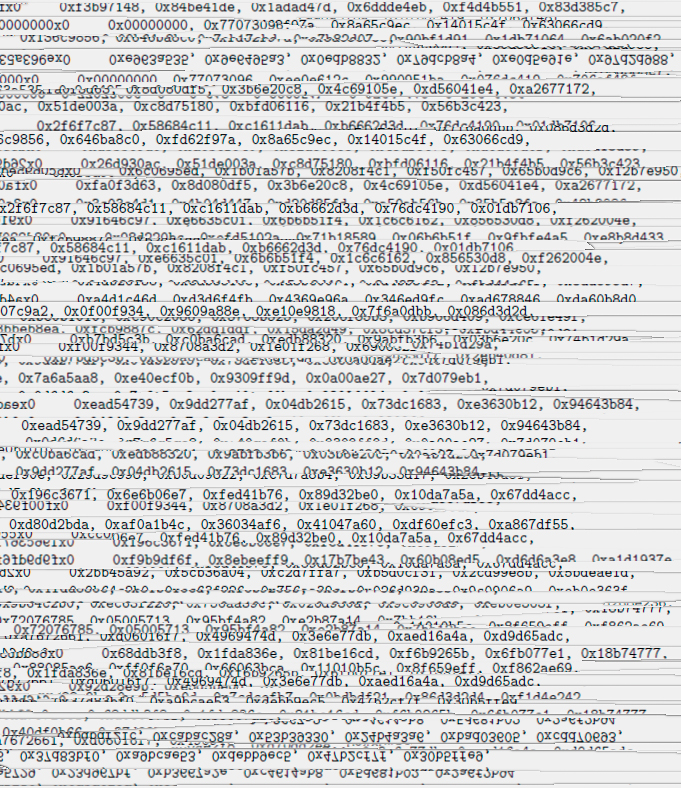
\includegraphics[scale=\FigScale]{cover.jpg}
\end{figure}

\bigskip

\hfill \huge \AUTHOR

\vspace*{\fill}
\end{center}

\end{titlepage}

\newpage

\begin{center}
\vspace*{\fill}
{\LARGE \TITLE}

\vspace*{\fill}

{\large \AUTHOR}

{\large \TT{<\EMAIL>}}
\vspace*{\fill}
\vfill

\ccbyncnd

\textcopyright 2013-2015, \AUTHOR. 

\RU{Это произведение доступно по лицензии Creative Commons «Attribution-NonCommercial-NoDerivs» 
(«Атрибуция~—~Некоммерческое использование~—~Без производных произведений») 3.0 Непортированная. 
Чтобы увидеть копию этой лицензии, посетите}%
\EN{This work is licensed under the Creative Commons Attribution-NonCommercial-NoDerivs 3.0 Unported License. 
To view a copy of this license, visit}%
\ES{Esta obra est\'a bajo una Licencia Creative Commons Atribuci\'on-NoComercial-SinDerivadas 3.0 Unported
Para ver una copia de esta licencia, visita}%
\PTBRph{}%
\PLph{}%
\ITAph{}
\url{http://creativecommons.org/licenses/by-nc-nd/3.0/}.

\RU{Версия этого текста}%
\EN{Text version}%
\ES{Versi\'on del texto}%
\PTBRph{}%
\PLph{}%
\ITAph{}
({\large \today}).

\RU{Самая новая версия текста (а также англоязычная версия) доступна на сайте}%
\EN{The latest version (and Russian edition) of this text is accessible at}%
\ES{La \'ultima versi\'on (as\'i como las versiones en ingl\'es y ruso) de este texto est\'a disponible en}%
\PTBRph{}%
\PLph{}%
\ITAph{}
\href{http://go.yurichev.com/17009}{beginners.re}.
\ifdefined\ebook
\RU{Версия формата A4 доступна там же.}
\EN{An A4-format version is also available.}
\ES{Una versi\'on en formato A4 tambi\'en est\'a disponible.}%
\PTBRph{}%
\PLph{}%
\ITAph{}
\else
\RU{Версия для электронных читалок так же доступна на сайте.}%
\EN{An e-book reader version is also available.}%
\ES{Una versi\'on para lector de libros electr\'onicos tambi\'en est\'a disponible.}%
\PTBRph{}%
\PLph{}%
\ITAph{}
\fi

\ifx\LITE\undefined
\RU{Существует также LITE-версия (сокращенная вводная версия), предназначенная для быстрого ознакомления
с основами reverse engineering:}%
\EN{There is also a LITE-version (introductory short version), intended for those who want a 
very quick introduction to the basics of reverse engineering:}%
\ES{Tambi\'en existe una versi\'on LITE (versi\'on corta e introductoria), dirigida a aquellos
que busquen una introducci\'on r\'apida a los fundamentos de la ingenier\'ia inversa:}%
\PTBRph{}%
\PLph{}%
\ITAph{}
\href{http://go.yurichev.com/17358}{beginners.re}
\fi

\RU{Вы также можете подписаться на мой twitter для получения информации о новых версиях этого текста:}%
\EN{You can also follow me on twitter to get information about updates of this text:}%
\ES{Adem\'as puedes seguirme en twitter para obtener informaci\'on sobre actualizaciones de este texto:}%
\PTBRph{}%
\PLph{}%
\ITAph{}
\TT{@yurichev}\footnote{\href{http://go.yurichev.com/17021}{twitter.com/yurichev}},
\RU{либо подписаться на список рассылки}%
\EN{or subscribe to the mailing list}%
\ES{o subscribirte a la lista de correo}%
\PTBRph{}%
\PLph{}%
\ITAph{}%
\footnote{\href{http://go.yurichev.com/17020}{yurichev.com}}.

\RU{Обложка нарисована Андреем Нечаевским:}%
\EN{The cover was made by Andy Nechaevsky:}%
\ES{La portada fue hecha por Andy Nechaevsky:}%
\PTBRph{}%
\PLph{}%
\ITAph{}
\href{http://go.yurichev.com/17023}{facebook}.

\end{center}
